A indústria de jogos digitais cresce mais a cada dia, de acordo com a consultora Newzoo \space\cite{quanto_games_vao_movimentar} essa indústria tende a ultrapassar em 2023 os US\$ 200 bilhões (aproximadamente R\$ 1 trilhão). Novos jogos são produzidos e publicados diariamente e somente na plataforma digital Steam, foram publicados 10.963 novos títulos em 2022\space
\cite{numero_de_jogos_publicados_na_steam}.

Ademais, o mercado de jogos no Brasil teve um aumento de 2,5\% em 2022, conforme apontado por uma pesquisa sobre o crescimento da demanda \space \cite{pesquisa_games_brasil}. O custo de produção de jogos varia bastante, dependendo do tamanho e da complexidade do projeto, \emph{e.g.}, a empresa Rockstar Games revelou que o jogo Grand Theft Auto V custou cerca de 265 milhões de dólares para ser produzido e comercializado \space
\cite{gta_quanto_custou}.

Ainda, os mapas desempenham um papel fundamental nos jogos, fornecendo orientação aos jogadores e criando a sensação de escala em uma área. Por exemplo o jogo de aventura pirata chamado Sea of Thieves, os mapas revelam locais de interesse, como tesouros escondidos, missões e áreas perigosas. Eles ajudam os jogadores a planejar suas estratégias, explorar o mundo virtual e tomar decisões com base em informações espaciais. Além disso, os mapas podem transmitir a sensação de escala e proporção, dando aos jogadores uma compreensão visual da extensão do mundo do jogo. Portanto os mapas enriquecem a experiência geral do jogo, mas criar cenários pode ser um desafio especialmente levando em consideração o orçamento disponível \cite{video-game-maps, lecafedugeek}.

\begin{figure}[H]
	\caption{Mapa de tesouro do jogo Sea of Thieves}
	\centering % para centralizarmos a figura
	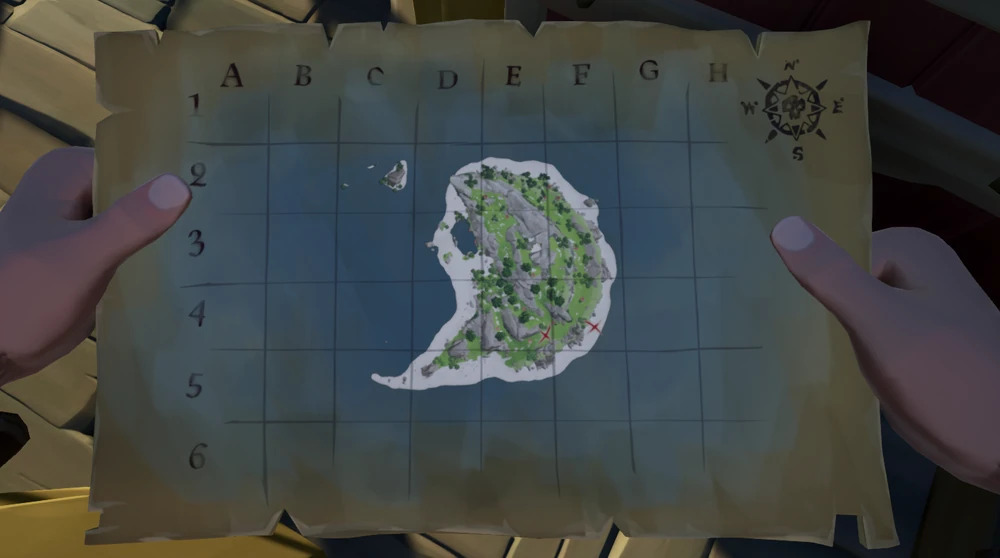
\includegraphics[width=10cm]{figures/Treasure_Map.jpg} % leia abaixo
	\legend{Fonte: \citeonline{seaofthieves}}
	\label{fig:treasureMap}
\end{figure}

Uma abordagem eficiente para resolver o problema é a geração procedural de mapas, que consiste em criar mapas usando algoritmos, tornando o jogo mais dinâmico e menos repetitivo. No entanto, a criação de cenários visualmente atraentes e diversos usando esse método ainda é um desafio \cite{geracao_procedural_jogos_2d}.

Contextualizando, a área de Geometria Computacional é um ramo da ciência da computação que estuda algoritmos e estruturas de dados para resolução computacional de problemas geométricos e o diagrama de Voronoi é um dos tópicos mais discutidos dessa 
área \cite{diagrama_voronoi_jogos}. O diagrama de Voronoi é gerado a partir das distâncias euclidianas entre os vizinhos mais próximos de um conjunto de pontos do plano\space\cite{diagrama_de_voronoi:_uma_exploracao_nas_distancias_euclidiana_e_do_taxi}. Esse diagrama possui uma gama de utilizações e dentre elas pode ser utilizado para resolver alguns problemas relacionados à jogos como por exemplo marcar pontos no mapa e desses pontos criar regiões, a partir dessas regiões criar biomas para serem usados no algoritmo de geração procedural de conteúdo para criar mapas.

De acordo com \citeonline{jogo_procedural} é muito comum em jogos usar técnicas procedurais para otimizar o processo de criação combinado com inteligência artificial para melhorar ou personalizar a experiência do jogador. Por exemplo, o jogo RimWorld é um simulador de colônia que utiliza uma IA para gerar histórias de forma procedural, abrangendo aspectos como psicologia, ecologia, combate e diplomacia, dentre outros \cite{jogo_procedural}.

A aplicação da IA em jogos não se limita apenas à jogabilidade. Ela também é usada em áreas como animação de personagens, reconhecimento de fala e expressões faciais, tradução automática de idiomas nos diálogos do jogo e muito mais. A IA está impulsionando a inovação e a evolução dos jogos, proporcionando experiências cada vez mais envolventes e cativantes para os jogadores \cite{exameNvidia, omniverseace}.

Ao explorar a relação entre IA e jogos no contexto da geração procedural de mapas, este trabalho contribuirá para a compreensão e o avanço dessa importante área de pesquisa, oferecendo aos jogadores experiências mais ricas e variadas. Dito isso, nosso projeto tem a ideia de fornecer recursos baseados em matemática aplicada dentro de ciência da computação que proporcione uma funcionalidade  de escolher o contorno do mapa no qual irá jogar através de imagens. Abordaremos a arquitetura de redes neurais convolucionais, que é muito utilizada para trabalhar com imagens. Mais especificamente, abordaremos uma arquitetura derivada da anteriormente citada, específica para segmentação de imagens, o que possibilita classificar contornos em imagens.

\section{Objetivos}

O objetivo geral deste trabalho é segmentar imagens utilzando uma arquitetura de redes neural convolucional e a partir do objeto selecionado gerar um mapa com uma aplicação procedural a partir do resultado do diagrama de Voronoi.
Ademais visto especificamente temos como objetivos:

\begin{itemize}
	\item Encontrar um conjunto de dados para treinar a inteligência artificial que irá identificar contornos em imagens
	\item Treinar uma inteligência artificial para identificar contornos em imagens
	\item Testar algoritmos de gerar ruídos para criar o mapa
	\item Aplicar um algoritmo para reconhecer a imagem com o contorno e gerar como saída a imagem do mapa gerado
\end{itemize}

% Outro cenário que está crescendo muito nos últimos anos é o da inteligência artificial, afirma \citeonline{Valente_2020} que no Brasil mais que dobrou o número contratações de desenvolvedores da área de 2015 até 2020. De acordo com \apud{johnson2023}{briggs2023} um relatório recente relata que 300 milhões de empregos podem ser afetados pela IA \emph{i.e.} 18\% ofício global pode ser automatizado. Outrossim \citeonline{europarl2020} diz que o tópico de inteligência artificial é uma prioridade para União Europeia por ser considerada primordial para transformação digital da sociedade.  Do mesmo modo, Bill Gates, um dos fundadores da Microsoft — uma das maiores empresas de tecnologia —, diz que "o desenvolvimento da inteligência artificial (IA) é o avanço tecnológico mais importante em décadas"\space
% \cite{inteligencia_artificial_e_avanco_bbc}.